
\documentclass[11pt]{book}
\usepackage{geometry}                % See geometry.pdf to learn the layout options. There are lots.
\geometry{letterpaper}                   % ... or a4paper or a5paper or ...
%\geometry{landscape}                % Activate for for rotated page geometry
%\usepackage[parfill]{parskip}    % Activate to begin paragraphs with an empty line rather than an indent
\usepackage{graphicx}
\usepackage{amsmath}
\usepackage{bm}
\usepackage{amssymb}
\usepackage{epstopdf}
\usepackage{microtype}
\usepackage{nicefrac}
\usepackage[pagestyles,raggedright]{titlesec}
\usepackage{xr}
\externaldocument{LabBook_Fall}

\setlength{\textheight}{625 pt}

\renewcommand{\chaptername}{}
\renewcommand{\thechapter}{}
\renewcommand{\thesection}{}
\renewcommand{\thesubsection}{}

% Tables stuff
\usepackage[table]{xcolor}
\usepackage{booktabs}
\usepackage{array}
\newcolumntype{L}[1]{>{\raggedright\let\newline\\\arraybackslash\hspace{0pt}}m{#1}}
\newcolumntype{C}[1]{>{\centering\let\newline\\\arraybackslash\hspace{0pt}}m{#1}}
\newcolumntype{R}[1]{>{\raggedleft\let\newline\\\arraybackslash\hspace{0pt}}m{#1}}

\DeclareGraphicsRule{.tif}{png}{.png}{`convert #1 `dirname #1`/`basename #1 .tif`.png}

\title{\bf{LABORATORY MANUAL}}
\author{DEPARTMENT OF PHYSICS\\
FAIRFIELD UNIVERSITY\\
\\
FALL 2019}
%\date{}                                           % Activate to display a given date or no date
%
%
%% titlesec stuff
\newpagestyle{main}{%
  \headrule
  \sethead[\chaptertitle][][]{}{}{\chaptertitle}
  \setfoot[\thepage][][]{}{}{\thepage}
}
\pagestyle{main}

% This option removes the Section Number
\setcounter{secnumdepth}{-2}

\setlength{\itemsep}{-5pt}

\begin{document}

\maketitle
%\tableofcontents
%
%%%%%%%%%%%%%%%%%%%%%
%                  %
%    Introduction  %
%                  %
%%%%%%%%%%%%%%%%%%%%

\labChapter{ii}{Introduction}



All scientists and engineers, whatever their field, use fairly standard procedures to record and analyze experimental data.
One key objective of this laboratory is that students explore the experiments using scientific methods that are common to all experiments, both in this laboratory and beyond.

The clear and correct presentation of experimental data is one of the highest priorities in science and engineering ethics.
Any claims made about experimental results must be supported through accurate measurements with related uncertainties and effective analysis.

Several concepts are important in obtaining and conveying scientific data.
\begin{enumerate}
  \item one must be able to accurately measure the variables of interest (for example, length, weight, or time) and know the limitations of those measurements.
  \item one must manipulate and convey that data in a manner that reflects the accuracy and precision of the measurements.
  \item one must be able to present the data in a format that is easily interpreted by the rest of the scientific community. Correct error analysis is critical in allowing the experimenter and others to draw valid conclusions from the results.
\end{enumerate}

In the sections at the end of this lab manual, we review the importance and use of significant figures, approaches to error analysis and the graphical representation of experimental data as well as an overview of how to use Vernier calipers for sub-millimeter length measurements.
A thorough review of this material (at the end of the manual) will greatly aid your ability to properly collect analyze and present your data in a post-laboratory submission.


 % Introduction
%%%%%%%%%%%%%%%%%%%%%
%                                              %
%                 Error Analysis               %
%                                              %
%%%%%%%%%%%%%%%%%%%%

\labChapter{}{Error Analysis}

In laboratory work, it is usually necessary to use experimental apparatus to measure physical quantities. The measurements are seldom, if ever, perfect. As a result, imperfections must be taken into account in any set of physical measurements. One of the most important things to be learned in the laboratory is how to make reliable estimates of the uncertainties involved in any physical measurements and how to handle the propagation of these errors, i.e., to know how the uncertainties affect calculated results of an experiment.


% Types of Errors
\section{Error Analysis Procedure}
\label{sec:ErrorProc}

This section is a guide to performing error analysis for an experiment.  The steps are detailed in the following sections.
\begin{itemize}
\item[\(\triangleright\)] Identify the likely sources of measurement error.
  \begin{itemize}
  \item Measurement errors can stem from the instrumentation, the experimental setup and procedure.
  \item Explain whether errors are systematic or random (\ref{sec:TypesErrors}).
  \end{itemize}
\item[\(\triangleright\)] Estimate the magnitude of the measurement errors using:
  \begin{itemize}
  \item the specification of the equipment,
  \item significant digits displayed,
  \item your estimate of how accurately you can read the instrument,
  \item the range or standard deviation of repeated measurements (\ref{sec:TypesErrors}).
  \end{itemize}
\item[\(\triangleright\)] Calculate the magnitude of the expected error in calculated experimental quantities due to your measurement errors (\ref{sec:ErrorPropagation}).
\item[\(\triangleright\)] If the difference between your results and expected results is much more than the magnitude of error you expect, look for a cause for the difference, including:
  \begin{itemize}
  \item a problem in how the experiment was performed,
  \item a calculation problem, a units conversion error, or using a trig function with degrees instead of radians,
  \item your estimate of the measurement error is too small,
  \item an error in some common value used in the calculations.
  \end{itemize}
\item[\(\triangleright\)] Report your results with the correct number of significant digits (\ref{sec:SigFig}) and with the calculated error.
\end{itemize}

\section{Types of Errors}
\label{sec:TypesErrors}

Experimental measurements are characterized by accuracy and precision. As illustrated in Fig.~\ref{fig:PreciseAccurate}, a set of measurements is precise and accurate if the average value of many measurements is close a known or expected value. A set of measurements is precise if they are closely clustered around their average value. Random errors cause more scatter in the results and reduce the precision of a measurement. Random measurement errors can be due to the inherent limitations of the equipment. They can be estimated and reduced by repeated measurements.  Systematic or precision errors can be due to equipment calibration or approximations in analysis. They reduce the precision of the experiment and are not reduced by repeated measurements. Often you can estimate precision errors by considering the equipment and its specifications.

\begin{figure}%[htbp] %  figure placement: here, top, bottom, or page
  \begin{center}
    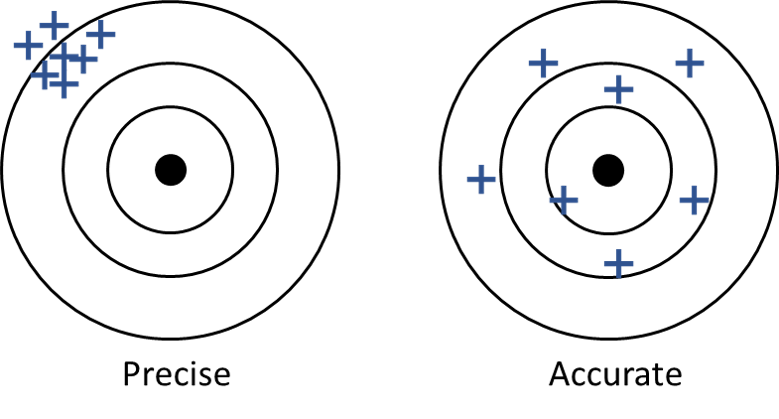
\includegraphics[width=3in]{{IntroductionFigures/ErrorType.png}}
  \end{center}
  \caption{The distinction between precision and accuracy.}
  \label{fig:PreciseAccurate}
\end{figure}

Error analysis can help you recognize if your results are consistent with a known or expected value. Each measurement has some combination of systematic and random errors. Make your best estimate of the possible error in each measured value. Your estimate may include instrument limitations and variation of measurements over multiple trials. Calculate the differences between your experimental results and any known values. Recalculate the experimental value in your spreadsheet by changing your measurements by adding or subtracting the estimated errors. Observe the range of experimental values (maximum and minimum) that you find in these recalculations.  If the expected values fall too far outside this range, there is some problem which you need to address.

Suppose you are measuring the density of a rectangular block. The block has dimensions $L=2.00\,\centi\meter$,  $ W=3.00\,\centi\meter$ and $H=5.00\,\centi\meter$. The mass of the block is $M=60.00\,\gram$. The uncertainty in the length measurements is $\pm0.01\,\centi\meter $ and the uncertainty in the mass is $\pm0.05,\gram$. The calculated density is mass divided by volume. The value calculated directly from your measurements is $\rho_{\mbox{expt}} = \nicefrac{60.00\,\gram}{30.00\,\centi\meter\cubed} = 2.00\,\gram\per\centi\meter\cubed $. The maximum density consistent with your measurements is the ratio of the maximum mass and the minimum volume: \(\rho_{\mbox{max}} = \nicefrac{60.05\,\gram}{\left(1.99\times0.99\times4.99\,\centi\meter\cubed\right)} = 2.02\,\gram\per\centi\meter\cubed\). Similarly, the minimum density consistent with your result is $1.98\,\gram\per\centi\meter\cubed$. If the expected density is not in this range, you need to consider possible explanations: the errors in the measurements could be larger than you estimated, the actual density could be different from the expected value, your calculation may be wrong, or perhaps the shape is not exactly rectangular.

The two types of errors illustrated in Fig.~\ref{fig:PreciseAccurate} require different treatment. The systematic errors illustrated on the target labelled ``Precise'' cannot be reduced by taking more measurements, while the average value obtained with the random errors on the target labelled ``Accurate'' improves with more measurements. The following sections provide guidance on analyzing systematic and random errors.

% Random Errors
\subsection{Random Errors}
\label{sub:RandomErrors}

Random errors are inherent in almost all measurements. They arise because of uncontrollable conditions affecting the observer, the measuring device, and the quantity to be measured. On the basis of probability it is assumed that these errors are as likely to be positive as negative, and more likely to be small than large. Taking a number of independent measurements of a given physical quantity and using the arithmetic average of these values in any computation may therefore minimize their effect. This minimization is only achieved if the measurements are independent. A common mistake is biasing a new measurement to agree with the previous measurements. This mistake makes the measurements more precise, but less accurate as shown in Fig.~\ref{fig:PreciseAccurate}. Taking truly independent measurements is the best way to reduce random error.

%The precision with which a physical quantity has been measured depends upon the spread of the set of measurements about their mean value. If the separate measurements are widely dispersed about the mean, the precision is low.  If the separate measurements are all close, the precision is high. There are many methods of estimating the spread of a set of measurements about the mean value. In general, one usually determines the deviations of the measured values from the mean value and then uses some function of these deviations to represent the spread, and thus the precision of the set of measurements.

The most well established method to quantify the spread of random errors in a measurement is to compute the {\it standard deviation}. Suppose you make $N$ measurements $x_1$, $x_2$, \ldots, $x_N$ of a certain quantity $x$. The average value is
\begin{equation}
  \label{eq:errorMeanX}
  \bar{x}=\frac{x_1 + x_2 + \ldots + x_N}{N}=\frac{1}{N}\sum_{i=1}^N x_{i},
\end{equation}
and the standard deviation of the individual measurements is
\begin{equation}
  \label{eq:errorSigmaX}
  \sigma = \sqrt{\frac{(x_1-\bar{x})^2 + (x_2-\bar{x})^2 + \ldots + (x_N-\bar{x})^2}{N-1}} = \sqrt{\frac{1}{N-1} \sum_{i=1}^{n}\left(x_i-\bar{x}\right)^2}.
\end{equation}
In Excel these operations can be carried out using the functions \texttt{AVERAGE()} and \texttt{STDEV()} or \texttt{STDEV.S()}.

If you perform many measurements, then your estimate of the average value improves. The ``standard deviation of the mean'' for $N$ measurements is
\begin{equation}
  \label{eq:errorSigmaMeanX}
  \sigma_{\mbox{mean}} = \frac{\sigma}{\sqrt{N-1}}.
\end{equation}
Your best estimate of a measurement $x$ is then $\bar{x} \pm \sigma_{\mbox{mean}}$.

For example, suppose that four measurements of a length yield, in centimeters, 7.65, 7.61, 7.66, 7.68.  The mean value is
\[
\bar{x} = \left(7.65 + 7.61 + 7.66 + 7.68\right)/4\,\centi\meter
        = 7.65\,\centi\meter,
\]
and the standard deviation is
\[
\sigma = \sqrt{\frac{(7.65-7.65)^2 + (7.61-7.65)^2 + 
                     (7.66-7.65)^2 + (7.68-7.65)^2}{4-1}\centi\meter\squared}
       = 0.029\,\centi\meter.
\]
The standard deviation of the average value is thus reduced to $ 0.029\,\centi\meter / \sqrt{3} =  0.017\,\centi\meter $ and therefore the best estimate of the length is $\bar{x} =  7.65\,\centi\meter \pm 0.017\,\centi\meter$.

%A simple but effective measure of the spread of indeterminate errors in the measurement of a quantity is the average deviation from the mean. Thus, if a given quantity is measured several times and the mean value of these measurements is computed, then the indeterminate error may be represented by the average difference between the mean value and the measured values without regard to sign. For example, suppose that four measurements of a length yield, in centimeters, 7.65, 7.61, 7.66, 7.68. The mean value is 7.65. The deviations without regard to sign are 0.00, 0.04, 0.01, 0.03. The average deviation from the mean is 0.02. If this average deviation is first subtracted from, and then added to, the mean value, an interval is defined (7.63 to 7.67), which generally brackets about half of the measured values. In this example the measurements 7.65 and 7.66 lie within the interval but 7.61 and 7.68 lie outside the interval. In many cases, it is desirable to extend the interval so as to include almost all the measured values, which can generally be done by using twice the average deviation as a measure of the indeterminate errors. The interval in the above example then becomes $7.65 \pm 0.04$ and includes all the measured values.

Frequently, a set of measurements has to be taken in an experiment under a prescribed condition. It may be difficult to judge exactly when this condition is satisfied. In this case, it may be necessary to vary the physical quantities that produce this condition and to note how much each may be varied without appreciably altering the prescribed condition. This variation may be used to determine the error.

Finally, the measuring devices (meter stick, voltmeter, and so on) are not perfectly accurate even if one could make a precise reading with them. The manufacturer specifies the accuracy in the measuring device; for example, a particular type of voltmeter may be guaranteed to give readings accurate to $\pm 1\%$ of full scale reading. Part of this tolerance is random error that can average out by taking multiple readings. As discussed in the next section, another part of the instrument error is systematic. An ammeter may always read $0.5\%$ high because of the value of a resistor internal to the device.

% Systematic Errors
\subsection{Systematic Errors}
\label{sub:SystematicErrors}

Systematic errors occur in an experiment because of a defective measuring apparatus, faulty methods, or incomplete working equations. They are definite in sign and magnitude and cannot be reduced by taking the average of a number of measurements, because the same error is included in each measurement.
These errors are often more important than the random errors. Calibrating the measuring apparatus, modifying the method, or changing the working equations may reduce them. These procedures are generally described as corrections that are to be made in performing the experiment.
For example, the reading of a Vernier caliper may not be zero when the jaws are in contact. This so-called zero error must be corrected for in using the instrument, i.e., the instrument must be calibrated. Otherwise, all measurements made with the caliper will be in error by a determinate amount, the zero error.

In many experiments time is measured with a stopwatch. Using a stopwatch that does not run at the proper rate would introduce an instrumental systematic error. A watch that ran too fast would cause all times recorded to be too high. A more significant systematic error encountered with a stopwatch is reaction time error. In measuring the time for an air track glider to travel down an incline, the observer may introduce a systematic error due to the reaction time required to stop the watch and a random error due to variation in reaction time. Report this source of error as ``reaction time error.'' The expression ``human error'' is too ambiguous to be useful in describing measurement errors.

%An example of personal systematic error is the tendency to look favorably at the first reading taken and then with suspicion on subsequent readings that differ. Other personal errors can be attributed to eyestrain, fatigue, or the position of the eye relative to a scale. Sloppy alignment of the end of a meterstick or failure to properly zero a balance are personal systematic errors which can be avoided with due diligence.

\subsection{Difference between Experimental Value and Expected Value}
\label{sub:ExperimentExpected}

If the true value of a quantity is known, then the systematic error can be estimated as difference between the result observed (experimental value) and the expected value. It is important to remember that this is an estimate of the systematic error. The difference between your experimental value and the expected value is \textbf{not an estimate of the random experimental error}. To report this difference as a percentage, divide the difference by the true value and multiply by 100\%. In Excel, use percent format instead of multiplying by 100\%.

%\begin{align} %
%        \%-\mbox{difference} = \frac{\mbox{Experimental Value} - \mbox{Actual Value}}{\mbox{Actual Value}} \, 100 \%
%\end{align}

If the true value of a quantity is known, then the difference between the experimental value and the expected value must be compared with the estimated systematic and random errors.  The difference between your experimental value and the expected value is \textbf{not an estimate of the experimental error}. To report this difference as a percentage, divide the difference by the true value and multiply by 100. In Excel, use percent format instead of multiplying by 100.

The percent difference between the experimental value and the expected value is
\[
\frac{\mbox{Experimental Value} - \mbox{Actual Value}}{\mbox{Actual Value}} \times 100\%.
\]
For example, suppose a student measures the value of gravity and finds it to be $9.41\,\meter\per\second\squared$, while the standard value is $9.803\,\meter\per\second\squared$.
The systematic relative difference, expressed as a percentage, is $\nicefrac{-0.39}{9.803} \times 100\% = -4.1\%$.
%The difference is $- 0.40 \meter\per\second\squared$.  It is important to maintain the proper sign of the error.
There is no definite allowable difference between the experimental and expected values in the following experiments. However, all measurements should be made with the greatest care, so as to reduce the error as much as possible.

It should be noted that the percent difference is not an estimate of experimental error. Any measurement has random and systematic errors even if the percent difference happens to be small.  Often, scientists do not know the actual value of the quantity they are measuring and they give their best estimate with error. Comparing the difference of the experimental value and the actual value with your best estimate of the experimental error will help determine if there is a systematic error in your results. If the difference is less than your estimated random error, then the results are consistent with the expected value. Having a zero percent difference could be the result of a lucky cancellation of errors and still just means the results are consistent. If the difference is significantly more than the estimated error, then you can begin to ask why your result is not consistent with the expected value.

% Propagation of Systematic Errors
\section{Propagation of Errors}
\label{sec:ErrorPropagation}

Through indirect measurement, the effect of systematic errors can be followed through the equations used. Two simple examples will be discussed.

% Calculation from a single, direct measurement
\subsection{Calculation from a Single, Direct Measurement}

Consider the volume of a sphere $V$ as calculated from a direct measurement of its diameter, $D$.  We would use
\[
  V = \frac{1}{6} \pi \, D^3
\]
where $\pi = 3.1415926\ldots$.  Suppose the value of $D$ is measured as $3.04\,\centi\meter$ and $V$ computed to be $14.71\,\centi\meter\cubed$. It is later discovered that the value of $D$ has a systematic error $\Delta D = +0.01\,\centi\meter$, (unnecessarily large, in all probability). What is the error $\Delta V$ in $V$ and the correct value of $V$?

\begin{enumerate}
\item Direct, brute-force method:\\
  Correct $D$ to $3.03\,\centi\meter$; re-compute $V_{\mbox{corr}}$ as $14.56\,\centi\meter\cubed$.\\
  The systematic error $\Delta V$ in $V$ is then $V - V_{\mbox{corr}} = 0.15\,\centi\meter\cubed$ or +1\%
\item Method based on calculus:\\
  Find the derivative of $V$ with respect to $D$,
  \begin{equation}
    \label{Eq:errorCalcMethod}
    \begin{aligned} %
      \frac{{\rm d}V}{{\rm d}D} &= \frac{3}{6} \pi D^2\\
           {\rm d}V             &= \frac{3}{6} \pi D^2 {\rm d}D.
    \end{aligned}
  \end{equation}
  Note that this shows a direct dependence of a change in $V$ on an infinitesimal change in $D$. Now divide through by $V = \frac{1}{6} \pi \, D^3$
  \[
    \frac{{\rm d}\,V}{V} = 3 \, \frac{{\rm d}\, D}{D}.
  \]
  If a finite change in $D$, such as the systematic error $\Delta D$, is small compared to $D$, then ${\rm d}\,V$ and ${\rm d}\,D$ can be approximated by $\Delta V$ and $\Delta D$, respectively, and so the following can be written:
  \[
    \frac{\Delta V}{V} \approx 3 \, \frac{\Delta D}{D}.
  \]
  This means that the fractional or percent error in $V$ is very nearly 3 times as large as that in $D$. Therefore,
  \[
    \frac{\Delta V}{V} \approx + 3 \, \frac{0.01}{3.04} \approx 1 \%.
  \]
  Hence,
  \[
    \Delta V \approx 0.15\,\centi\meter\cubed
  \]
  and
  \[
    V_{\mbox{corr}} = V - \Delta V = 14.56\,\centi\meter\cubed.
  \]
\end{enumerate}

\subsection{Calculation from Two or More Direct Measurements}

Consider the volume $V$ of a right, circular cylinder as calculated from its diameter $D$ and length $L$. For convenience, let $D$ be measured as $2.00\,\centi\meter$  and $L$ as $5.00\,\centi\meter$. Then,
\[
  V = \frac{1}{4} \pi \, L \, D^2 = 15.71\,\centi\meter\cubed.
\]
If $D$ has an error of $+0.01\,\centi\meter$ and $L$ an error of $-0.02\,\centi\meter$, what is the error $\Delta V$ in $V$ and what is the correct value of $V$?
\begin{enumerate}
\item Direct, brute-force method:\\
  To obtain $V_{\mbox{corr}}$, subtract $0.01\,\centi\meter$ from $D = 2.00\,\centi\meter$, add $0.02\,\centi\meter$ to $L = 5.00\,\centi\meter$ and recompute $V_{\mbox{corr}}$ as $15.61\,\centi\meter\cubed$, whereby $\Delta V$ must be $+0.01\,\centi\meter\cubed$.

\item Method based on calculus:\\
  Find the partial derivatives of $V$
  \[
    \frac{\partial V}{\partial L} =\frac{1}{4} \pi \, D^2   \hspace{2 cm}   \frac{\partial V}{\partial d} =\frac{1}{2} \pi \, D \, L
  \]
  \[
    {\rm d}\, V = \frac{\partial V}{\partial L} \, {\rm d}\, L + \frac{\partial V}{\partial D} \, {\rm d}\, D
  \]
  so that
  \[
    \Delta V \approx \frac{\partial V}{\partial L} \, \Delta L + \frac{\partial V}{\partial D} \, \Delta D = \frac{\pi}{4} \, D^2 \, \Delta L + \frac{\pi}{2} \, D \, L \, \Delta D.
  \]
  Now dividing through by $V = \frac{1}{4}\pi \, D^2 \, L$
  \[
    \frac{\Delta V}{V} \approx \frac{\Delta L}{L} + \frac{2 \Delta D}{D}.
  \]
  i.e.\ the fractional (or percent) systematic error in $V$ is very nearly equal to the fractional systematic error in $L$ plus twice the fractional error in $D$.  In our case,
  \[
    \frac{\Delta L}{L} = \frac{-0.02}{5.00} = -0.4 \%
  \]
  and
  \[
    \frac{2\Delta D}{D} = \frac{+0.02}{2.00} = +1.0 \%
  \]
  so that
  \[
    \frac{\Delta V}{V} \approx +0.6 \%.
  \]

  Thus $\Delta V = +0.09\,\centi\meter\cubed $, i.e.\ the systematic error, is  $+0.09\,\centi\meter\cubed$, the correction is $-0.09\,\centi\meter\cubed$ and $V_{\mbox{corr}} = +15.62\,\centi\meter\cubed $.
\end{enumerate}
% Significant Figures

\section{Significant Figures}
\label{sec:SigFig}

The number of digits required to express the result of an experimental measurement, so that it reflects the accuracy with which the measurement was made, are known as significant figures. Thus, the number of significant figures reflects the limitation of the measuring device and/or the experimenter. Whether the calculations are performed by hand or on a computer, the number of significant figures displayed in the final result must reflect the limitations of the experimental measurement. Often, a computer program will, by default, display either too many or too few digits. If too few digits are displayed, you need to adjust the program setting to show more digits.

For example, if the length of a cylinder is measured as $20.64\,\centi\meter$, this quantity is said to be measured to four significant figures.  If written as  $0.0002064\,\kilo\meter$, we still have only four significant figures. The zeros preceding the ``2'' are used only to indicate the position of the decimal point. The zero between the ``2'' and the ``6'' is a significant figure, but the other zeros are not.  If the above measurement is made with a meter stick, the last digit recorded is an estimated figure representing a fractional part of a millimeter division. All recorded data should include the last estimated figure in the result, even though it may be zero. If this measurement had appeared to be exactly $20$, it should have been recorded as $20.00\,\centi\meter$, since lengths can be estimated by means of this instrument, to about $0.01\,\centi\meter$. When the measurement is written as $20\,\centi\meter$ it indicates that the value is known to be somewhere between $19.5\,\centi\meter$ and $20.5\,\centi\meter$, whereas the value is actually known to be between $19.995\,\centi\meter$ and $20.005\,\centi\meter$.  Conversely, retaining too many significant figures implies greater accuracy than the figures actually represent.

When deciding the number of significant figures to retain, the following rules apply:
\begin{itemize}
	\item[\(\triangleright\)] When collecting data, only one estimated figure is retained as a significant figure.
	\item[\(\triangleright\)] In addition and subtraction, do not carry the result beyond the first column that contains an estimated figure. All figures lying to the right of the last column in which all figures are significant should be dropped.
	\item[\(\triangleright\)] In multiplication and division the result should have as many significant figures as the factor with the least number of significant figures.
	%(In some instances, the result should have one more significant figure than the factor with the least number of significant figures. For example, in the equation $8.5 \times 1.48 = 12.6$, if the result is to be as accurate as the least accurate of the factors, three significant figures are needed even though the factor with the least number of significant figures has two.)
	\item[\(\triangleright\)] When dropping figures that are not significant, round to the nearest significant digit.  That is to say, the last figure should be unchanged if the first figure dropped is less than 5.  The last figure retained should be increased by one if the first figure dropped is 5 or greater.
	\item[\(\triangleright\)] While performing intermediate calculations, it is safer to carry one more significant figure than is required in the final result.  You can always fix it when you're done.
\end{itemize}
The following examples help illustrate these rules.

When adding these four numbers
\begin{equation*}
	\begin{aligned} %
		427&.5\\
		28&.03\\
		0&.0654\\
		396&.0\\
		\hline
		851&.6
	\end{aligned}
\end{equation*}
the result is written rounded to the first decimal digit, 851.6, because the first term in the sum is only given to one decimal digit. The sum is expressed to the proper number of significant figures.

In our next example, we will calculate the area of a rectangle. The length is measured as $1.94\,\centi\meter$, and the width as $1.84\,\centi\meter$. A calculator provides the result of $3.5696\,\centi\meter\squared$. This number has five significant figures while each of the factors has three significant figures. Therefore, the result should have three significant figures and is expressed as $3.57\,\centi\meter\squared$.

In Excel, the number of significant figures can be set by formatting the cell to a ``Number'' type with the desired number of decimal places. In addition to being more meaningful, formatting the cells makes the spreadsheet more readable.
 % ErrorAnalysis
%%%%%%%%%%%%%%%%%%%%%%%%%%%
%                                                        %
%                Graphical Representation                %
%                                                        %
%%%%%%%%%%%%%%%%%%%%%%%%%%

\labChapter{}{Graphical Representation of Experimental Data}

From an examination of the tabulated values of a number of measurements of related quantities, it is often difficult to grasp the relationships existing between the numbers. A method widely used to discover such relationships is the graphical method, which gives a pictorial view of the results and makes it possible to interpret the data by a quick glance.

% Independent and Dependent Variables
\section{Independent and Dependent Variables}

In any experimental study of cause and effect the aim is to vary just one condition at a time (the cause) and to observe the corresponding values of another quantity (the effect), which is suspected of being related to the first. The existing relationship is most easily interpreted from the graph if the first of these quantities, the independent variable, is plotted on the abscissa scale ($x$-axis), and the dependent variable is plotted on the ordinate scale ($y$-axis). For example,
\[
y = f(x)
\]
means that for each value $x$, the independent variable, there is a corresponding value of $y$, or, $y$ is a function of $x$.

Graphs should have the following features:
\begin{itemize}
\item[$\triangleright$] Axes tick marks and axis labels indicating the numerical scale  of the quantity,
\item[$\triangleright$] Axes titles with the name of the quantity and the units,
\item[$\triangleright$] A descriptive graph title,
\item[$\triangleright$] Points should not be joined by lines and there is no need to label them with the actual values, and
\item[$\triangleright$] If possible, the full scale should be visible and axes should intersect at $(0,0)$.
\end{itemize}
An example of how a graph should look is shown in Fig.~\ref{fig:graph}.

\begin{figure}%[htbp] %  figure placement: here, top, bottom, or page
  \begin{center}
    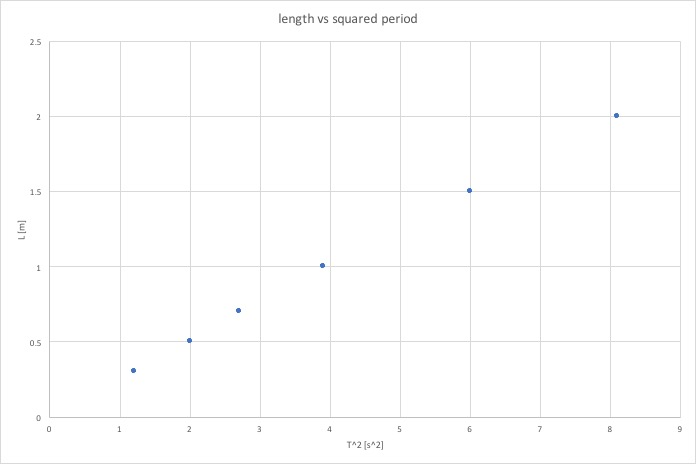
\includegraphics[width=4in]{IntroductionFigures/graph.jpg}
  \end{center}
  \caption{Example of a graph for the pendulum experiment showing the length as a function of the period squared.}
  \label{fig:graph}
\end{figure}

% Producing Graphs
\section{How to Produce Graphs}

There are many ways to produce graphs and just as many computer programs that will aid in the representation of data. This section will give simple instructions on how to make data graphs, using Excel.

\begin{itemize}
\item[$\triangleright$] Using a spreadsheet, it's easiest if you create a separate data table for each graph you want to make. By default Excel expects the first column of the table to be the values for the $x$-axis and the second column the values for the $y$-axis.
\item[$\triangleright$] Highlight \textit{both} columns and select \textbf{Charts} from the toolbar menu. Select the \textbf{Scatter} type and Excel will automatically produce the graph in your spreadsheet.
\item[$\triangleright$] You need to add labels and units to both axes by selecting the option \textbf{Axis Titles} in Excel and then edit the title by clicking on it.
\item[$\triangleright$] Very often you want to add a line-of-best-fit to your Excel graph. To do so follow the steps below:
  \begin{enumerate}
  \item In your graph, right-click (in Windows) or CTRL-click (on Mac) on one of the data points. This will open a pop-up menu. In this menu select \textbf{Add Trendline}. This will open a window with several items related to best-fit-lines and curves.
  \item Select the type of line you would like to add from the \textbf{Type} menu. If you want a straight line select \textbf{Linear}, for a polynomial (e.g.\ a parabola) select \textbf{Polynomial} and then the order will give the highest exponent (for a parabola the order would need to be a \textbf{2}).
  \item In the \textbf{Options} menu you can select two important options for the trend line:
    \begin{itemize}
    \item The \textbf{Set Intercept = \textit{value}} option will force the trendline to go through the point (0,\textit{value}). This is useful if you know that your curve is supposed to go through the origin. In this case set $\mbox{\textit{value}} = 0$ (the default value in Excel) and this forces the best-of-fit-line to go through the origin.
    \item The option \textbf{Display Equation on Chart} will print the equation of the trendline onto the chart. This is useful if you want to determine a value from your line-of-best-fit (e.g.\ the slope). You will have to select the equation and set the format to display the correct number of significant digits. The number of significant digits in an equation displayed on a chart is often too small, and sometimes rounded to 0 if values are small. Select the equation and under the format tab choose Format Selection and select scientific instead of general Alternatively, you can use the Excel functions \texttt{SLOPE()} and \texttt{INTERCEPT()}.  For more sophisticated fitting, the \texttt{LINEST()} function may be of use as well.
    \end{itemize}
  \end{enumerate}
\end{itemize}

Fig.~\ref{fig:graph2} shows again the length as a function of the period squared for a pendulum with a linear trendline. The line is the best fit to the points and the equation shows the resulting slope and intercept. Theoretically the intercept is expected to be zero and the slope is excepted to be $\nicefrac{4\pi^2}{g}=0.248\,\second\squared\per\meter$.  In Excel you can set the equation properties to force the intercept to zero. Often you need to reformat the displayed equation to show enough significant figures.

\begin{figure}%[htbp] %  figure placement: here, top, bottom, or page
  \begin{center}
    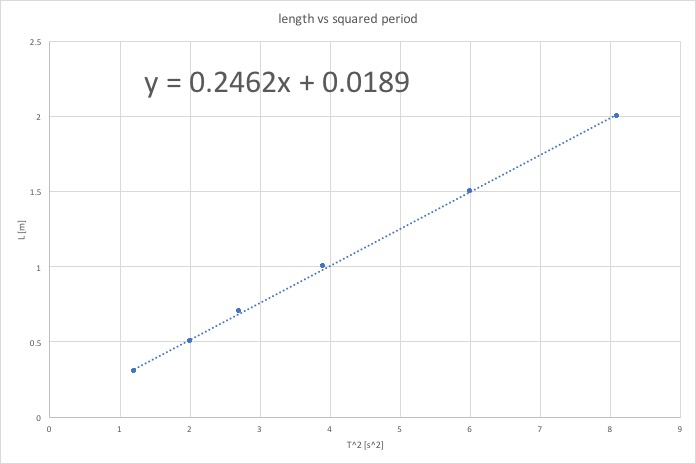
\includegraphics[width=4in]{IntroductionFigures/graph2.jpg}
  \end{center}
  \caption{Example of a graph with the trendline  and the corresponding equation.}
  \label{fig:graph2}
\end{figure}
 % GraphicalRepresentation
%%%%%%%%%%%%%%%%%%%%%
%                                             %
%                 Vernier Calipers            %
%                                             %
%%%%%%%%%%%%%%%%%%%%

\labChapter{}{Vernier Calipers}

The instrument illustrated in Fig.~\ref{VernierFig01} is a set of calipers.  The calipers have jaws $c$ and $d$ for measuring the diameter of a sphere or cylinder, $A$, or the thickness of any object placed between them. The inside diameter of a cavity is measured with jaws $e$ and $f$.  The depth of a hole is measured with the depth gauge, $g$.  The latter, and jaws $f$ and $d$ form part of a slide on which is engraved an auxiliary scale, the \textsl{Vernier scale} $v$. The scale on the fixed part (which carries jaws $c$ and $e$) is called the main scale. Only the metric scales are shown in the drawing, although the instrument have both U.S.\ and metric main and Vernier scales.

\begin{figure}
  \begin{center}
    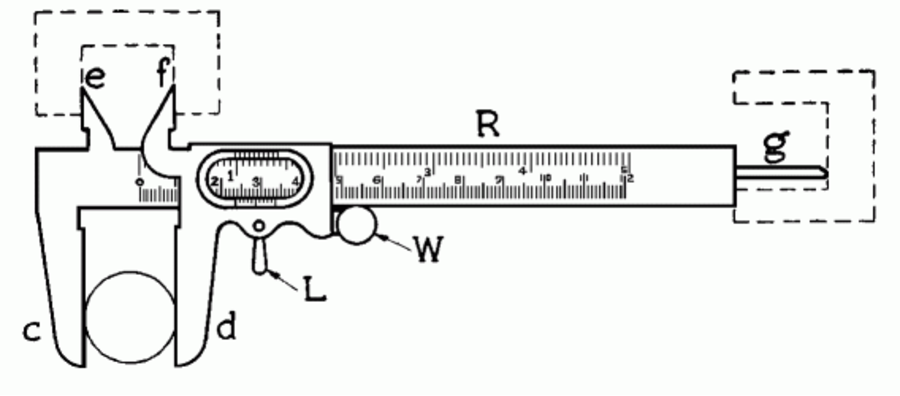
\includegraphics[width=5in]{IntroductionFigures/VernierCalipers01.pdf}
  \end{center}
  \caption{A diagram showing Vernier calipers and their main measurement scales.}
  \label{VernierFig01}  % the \label command comes AFTER the caption
\end{figure}

\section{Reading the Vernier scale}

Vernier scales, as used on the calipers and on many other types of high quality measuring instruments provide a means of reading accurately fractions of a scale division that otherwise have to be estimated.  In Fig.~\ref{VernierFig02}, we have illustrated a main scale with its Vernier scale.

\begin{figure}
  \begin{center}
    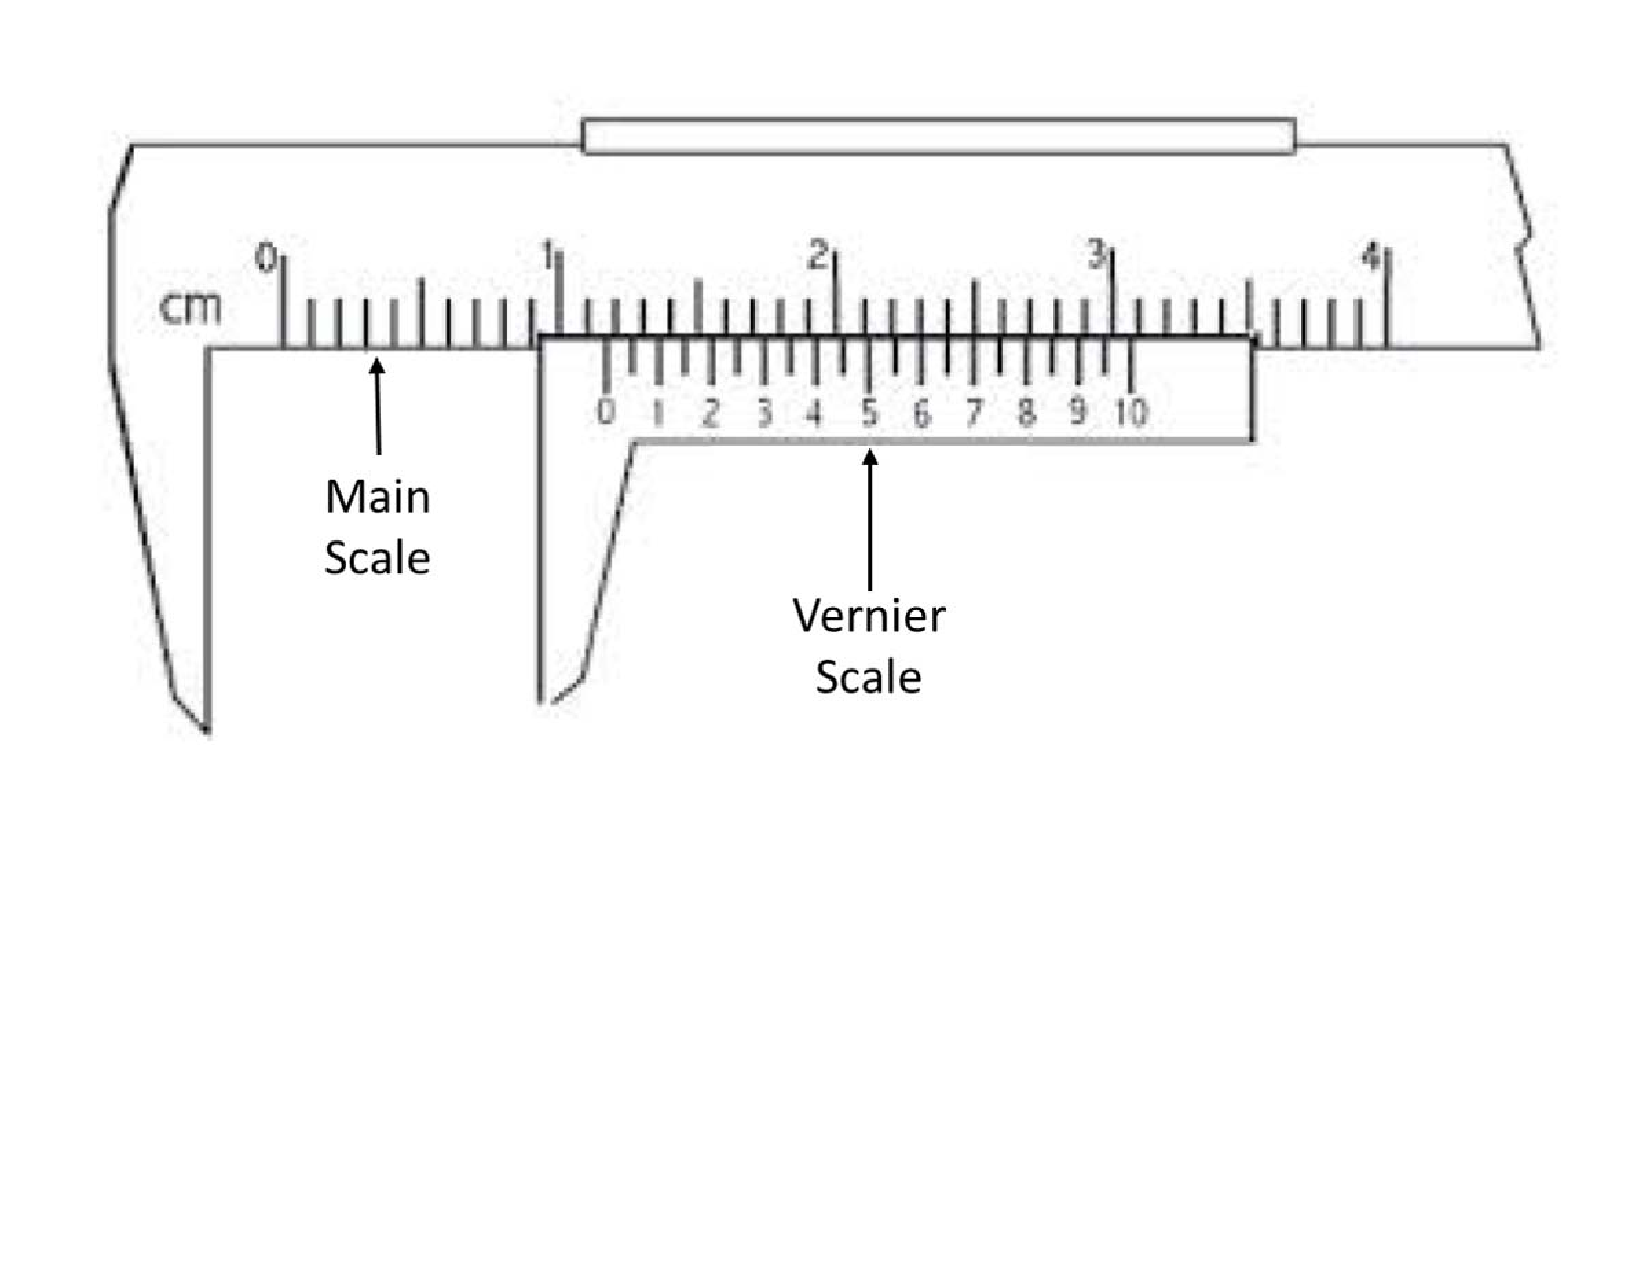
\includegraphics[width=5in]{IntroductionFigures/VernierCalipers02a.pdf}
  \end{center}
  \caption{How to read the value off the caliper slider.}
  \label{VernierFig02}  % the \label command comes AFTER the caption
\end{figure}

If each division on the main scale is $1\,\centi\meter$, then each division of the Vernier scale represents $1.0\,\milli\meter$.  Physically, it is a $9\,\milli\meter$ length divided into 10 equal parts. As an example, in the metric scale of Fig.~\ref{VernierFig02} the zero of the upper or Vernier scale is between the $1$ and $2\,\centi\meter$ marks on the main scale.  In this way, the Vernier scale is capable of interpolating to the nearest \milli\meter, the position of the Vernier zero mark on the main scale.  In this example, the measurement is  $1\,\centi\meter + \mbox{some number of \milli\meter}$.  In order to determine the number of \milli\meter, we read the number on the Vernier scale whose line coincides with a \centi\meter division line on the main scale.  (If the zero line of the Vernier is exactly on a division line of the main scale, then the measurement is exactly the main scale division.)  In this example, the division of the Vernier scale that lines up with a main scale division is the $0.7\,\milli\meter$ division.  The measurement would be $1.17\,\centi\meter$. You might have the situation where there is no exact alignment.  If that occurs, then you would estimate to the nearest $0.5\,\milli\meter$.  For example, if the $7\,\milli\meter$ division was slightly above and the $8\,\milli\meter$ division was slightly below corresponding marks on the main scale, then the measurement would be $1.175\,\centi\meter$.  Thus the Vernier scale is capable of estimating to the nearest $0.05\,\milli\meter$.  The rule for this type of Vernier therefore is to read the number of whole main scale divisions below the zero line of the Vernier, and in the next place of decimals insert the number of the line on the Vernier scale which coincides with a main scale line.

The smallest quantity, which may be read without estimating, is known as the least count; this is $1\,\milli\meter$ for the Vernier calipers illustrated.  For the Vernier calipers you will use in the laboratory, the least count is $0.1\,\milli\meter$.  In general, if the smallest division of the main scale of an instrument is $M$ units, and the length of the smallest Vernier division is $V$ units, then the least count, $L$, is $M V$. Also, since $n$ Vernier divisions are equal in length to $n-1$ main scale divisions,
\[
   nV = (n-1)M
\]
or
\[
   V = \frac{(n-1)M}{n}
\]
and thus
\[
   L = M - V = M - \frac{(n-1)M}{n} = \frac{M}{n}.
\]
 % VernierCalipers
%%%%%%%%%%%%%%%%%%%%%
%                                                %
%                 Data Acquisition               %
%                                                %
%%%%%%%%%%%%%%%%%%%%

\labChapter{}{Data Acquisition and Analysis}

%% Introduction
%\subsection{Introduction}

In this lab you will perform measurements and calculate results from the measurements. Each trial requires similar calculations.  The best way to perform repetitive calculation tasks is to use a computer program such as a spreadsheet. The effort to set up the calculation is more than compensated by the reliability and ease of repeating calculations. Several experiments will make use of sensors to aid in measurements and data gathering. The data in these experiments is collected by an advanced computer program called \textbf{Capstone}, which is installed on all computers in the lab. The program is also able to organize, analyze, and display the data. This section will give an overview of the program, explain how to set up sensors, and how to display data. More detailed information will be given in the specific experiments, which will make use of the sensors and data acquisition.

\section{Data Analysis with Spreadsheets}
\label{sec:dataSpreadsheet}

Data for each experiment has a set of measurements and calculations.
A spreadsheet is a grid of rows and columns where you can enter text, numerical values or formulas.
Spreadsheet programs provide all the mathematical functions, formatting, and graphing that you need for this lab.
You will often have a table of common values, another for measurements, and a table for summary calculations.
The standard way to structure a data analysis spreadsheet saves calculation errors and reduces repetitive typing.
Use a separate row for each trial and a separate column for each measured or calculated value.

\begin{itemize}
\item[$\triangleright$] Use a row for each trial, labeled in the left cell with, for example, ``Trial \#1''.
\item[$\triangleright$] Use a column for each measured or calculated value, labeled in the top cell with a description of the column and with units.
\item[$\triangleright$] Reference cells you need for a calculation. Do not retype numbers. Use \texttt{\$} for row or column coordinates you don't want to change. \texttt{\$D5} will always refer to column \texttt{D} but the row will change. \texttt{D\$5} will always refer to row 5 but the column will change. Finally, \texttt{\$D\$5} will always refer to the same cell.
\item[$\triangleright$] Never enter a value calculated outside the spreadsheet, for example, on your calculator. Any value you can find on the calculator can be calculated and updated automatically on the spreadsheet.
\item[$\triangleright$] Use the spreadsheet's ``fill down'' capability by selecting a set of cells in a row and fill down by dragging. Formulas will copy and the row numbers of referenced cells that are not preceded by \texttt{\$} will increment automatically.
\end{itemize}
This approach makes it efficient to create a spreadsheet to analyze your data and to correct errors. If you make a mistake in a formula, you can correct the first trial and then correct the other trials by filling down.

\section{Capstone}
\label{sec:SettingUpHardware}

May of our experiments use the \textsl{Capstone} program to
communicate with the measurment hardward and collect the data.  This
section is a very brief introduction to using the \textsl{Capstone}
software. 

% Setting up Hardware
\subsection{Setting up Hardware}

Once you have opened the program you will notice a button labeled \textbf{Hardware Setup} on the left-hand side of the main window. If you click on the button you will get a list of all sensors that are currently connected to the computer. In almost all cases the program will recognize the connected sensor automatically and load a standard setup for the corresponding sensor. In a few cases you will be required to provide the program with certain values needed to determine the value of the quantity the sensor is supposed to measure. In the specific instructions for the experiment you will be told what values to provide. If you do not see the sensor try to dis-  then reconnect the sensor to the computer or ask for help.

% Collecting Data
\subsection{Collecting Data}

Upon opening the \textbf{Capstone} program you have the choice of several display modes for the data you will be collecting. The exact choice depends on the experiment you will be performing and detailed instructions will be provided if they deviate from the description below. In the simplest of all cases you will be using the \textbf{Table \& Graph} display. If you click on this option the program will create a data table and a graph on the main canvas of the program. By default the measurements will be undetermined, but you can choose any variable that is allowed by the sensor to be displayed in the data table columns or on the graph axes. Clicking with the cursor onto the \textbf{Select Measurement} in the data table headers or on graph axes will allow you to chose the variable to display. At times a mathematical equation using the actual measured quantities can be defined by selecting the \textbf{Create New} \(\rightarrow\) \textbf{Calculation} (data table) or \textbf{Add Similar Measurement} (graph axes) option in the pulldown menus.

To start collecting data you need to press the red \textbf{Record} button on the bottom of the \textbf{Capstone} window. The program will then record all data being collected by the sensors and display them as numbers in the data table and points on the graph. The data collection can be stopped by pressing the red \textbf{Record} button a second time. After collecting all the data the information can then be analyzed.

% Analyzing Data
\subsection{Analyzing Data}

Data can be analyzed by exporting the collected data into a data file, that can be read by  Excel (or other mathematical program). An easier way to analyze the data is often to interpret the graph that has been produced by the \textbf{Capstone} program. Tools to analyze the graph are very readily available in the menubar above the graph window. The most important tools are discussed in more detail below:
\begin{itemize}
\item[\(\triangleright\)] \textbf{Highlight range of points in active data}.\\
This option allows you to consider only the highlighted region of the data set to be analyzed. Once selected the program will display a rectangular area that can be resized and dragged over the collected data points. Only the points inside the rectangle will be considered in the selected analysis tool. The selected points will also be displayed in the data table with the same highlighting.
\item[\(\triangleright\)] \textbf{Display selected statistics for active data}.\\
Selecting this option will display several useful mathematical quantities for the selected data set, e.g.\ average of all values, mean of all values, maximum value, minimum value, etc.
\item[\(\triangleright\)] \textbf{Display area under active data}.\\
This option will allow you to calculate the area under the curve for the selected data points (the integral).
\item[\(\triangleright\)] \textbf{Apply selected curve fits to active data}.\\
With this option the user can fit a line of best fit to the elected data range. The drop down menu will give several options for graphs to fit (e.g.\ straight line, parabola, etc.)
\item[\(\triangleright\)] \textbf{Show coordinates and access delta tool}.\\
Once selected this tool will display a cross-hair onto the coordinate frame and allow to determine the values of specific points by placing the cursor onto a data point of the graph. Right-clicking on the cursor will allow to select a delta tool to determine a range in the data set (both $x$- and $y$-range).
\end{itemize}
 % DataAcquisition
%\include{Experiment01} % M-1: Force Table included tilting the table in the procedure.
%\include{Experiment02} % M-2: Measurement of the Acceleration of an Object Due to Gravity
%\include{Experiment03} % M-3: The Measurement of ${\bm g}$ with a Simple Pendulum
%\include{Experiment08} % M-4: Centripetal Force
%\include{Experiment04} % M-5: Conservation of Energy
%\include{Experiment05} % M-6: The Ballistic Pendulum and Projectile Motion
%\include{Experiment06} % M-7: Conservation of Linear Momentum
%\include{Experiment09} % M-8: Rotational Motion
%\include{Experiment07} % M-9: Harmonic Motion
%\include{Experiment10} % H-1: Ideal Gas Law

\include{FallLabDataTables} % comment out to compile lab manual without tables
\end{document}
